
\documentclass{article}
\usepackage[utf8]{inputenc}
\usepackage{relsize}
\usepackage{amsmath}
\usepackage{geometry}
\usepackage{tikz}
\usetikzlibrary{automata, positioning, arrows}
\tikzset{node distance=2.5cm, % Minimum distance between two nodes. Change if necessary.
every state/.style={ % Sets the properties for each state
semithick,
fill=gray!10},
initial text={}, % No label on start arrow
double distance=2pt, % Adjust appearance of accept states
every edge/.style={ % Sets the properties for each transition
draw,->,>=stealth', % Makes edges directed with bold arrowheads
auto,semithick}}

\geometry{
 a4paper,
 total={170mm,257mm},
 left=20mm,
 top=20mm,
}

\title{Homework 2\\[0.2em]\smaller{}CSC 445-01: Theory of Computation}
\author{Matthew Mabrey, Luke Kurlandski}
\date{\today}

\begin{document}

\maketitle

\section*{1.12}

We describe $D$ more simply
$$D = \{w \big | w \textrm{  is a word with an odd number of } b \textrm{'s followed by an even number of } a \textrm{'s} \}$$
And construct a DFA that recognizes $D$
\begin{center}
    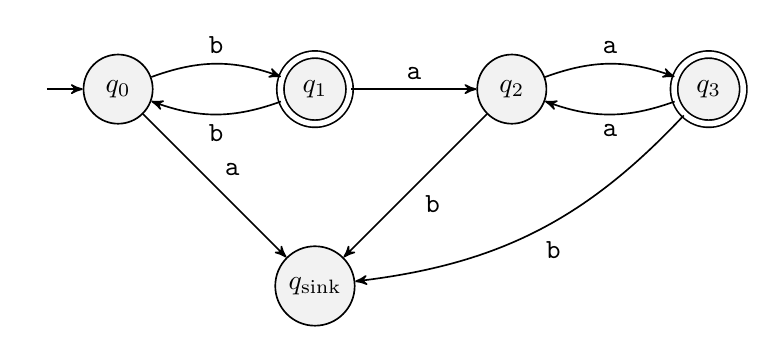
\begin{tikzpicture}
    
    \node[state, initial] (0) {$q_0$};
    \node[state, right of=0, accepting] (1) {$q_1$};
    \node[state, right of=1] (2) {$q_2$};
    \node[state, right of=2, accepting] (3) {$q_3$};
    \node[state, below of=1] (4) {$q_\textrm{sink}$};
    
    \draw (0) edge[bend left=20] node {\tt b} (1);
    \draw (1) edge[bend left=20] node {\tt b} (0);
    \draw (1) edge node {\tt a} (2);
    \draw (2) edge[bend left=20] node {\tt a} (3);
    \draw (3) edge[bend left=20] node {\tt a} (2);
    
    \draw (0) edge node {\tt a} (4);
    \draw (2) edge node {\tt b} (4);
    \draw (3) edge[bend left=20] node {\tt b} (4);
    
    \end{tikzpicture}
\end{center}

\section*{1.16 a}

\begin{center}
    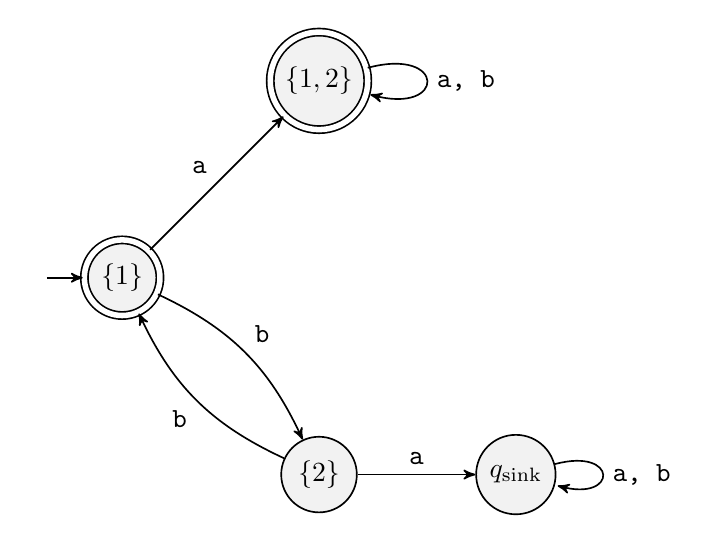
\begin{tikzpicture}
    
    \node[state, initial, accepting] (0) {$\{1\}$};
    \node[state, right of=0, below of=0] (1) {$\{2\}$};
    \node[state, right of=0, above of=0, accepting] (2) {$\{1, 2\}$};
    \node[state, right of=1] (3) {$q_\textrm{sink}$};
    
    \draw (0) edge[bend left=20] node {\tt b} (1);
    \draw (0) edge node {\tt a} (2);
    \draw (1) edge[bend left=20] node {\tt b} (0);
    \draw (1) edge node {\tt a} (3);
    
    \draw (2) edge[loop right] node {\tt a, b} (2);
    \draw (3) edge[loop right] node {\tt a, b} (3);
    
    \end{tikzpicture}
\end{center}

\section*{1.20 g}

For the regular expression $R = (\epsilon \cup a)b $\\\\
Members include
\begin{itemize}
    \item $b$
    \item $ab$
\end{itemize}
Non members include
\begin{itemize}
    \item $a$
    \item $aba$
\end{itemize}

\section*{1.21 a}

\begin{center}
    \begin{tikzpicture}
    
    \node[state, right of=0, initial] (1) {$1$};
    \node[state, right of=1, accepting] (2) {$2$};
    
    \draw (1) edge[bend left=20] node {\tt b} (2);
    \draw (2) edge[bend left=20] node {\tt b} (1);
    
    \draw (1) edge[loop above] node {\tt a} (1);
    \draw (2) edge[loop above] node {\tt a} (2);
    
    \end{tikzpicture}

    ~\\
    
    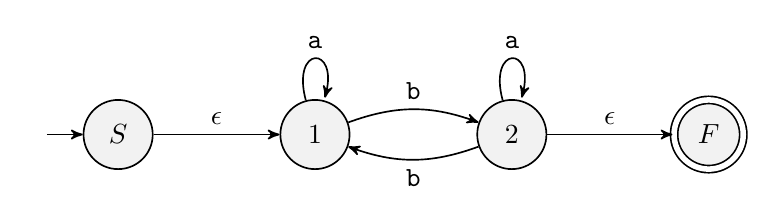
\begin{tikzpicture}
    
    \node[state, initial] (0) {$S$};
    \node[state, right of=0] (1) {$1$};
    \node[state, right of=1] (2) {$2$};
    \node[state, right of=2, accepting] (3) {$F$};
    
    \draw (1) edge[bend left=20] node {\tt b} (2);
    \draw (0) edge node {\tt $\epsilon$} (1);
    \draw (2) edge[bend left=20] node {\tt b} (1);
    \draw (2) edge node {\tt $\epsilon$} (3);
    
    \draw (1) edge[loop above] node {\tt a} (1);
    \draw (2) edge[loop above] node {\tt a} (2);
    
    \end{tikzpicture}
    
    ~\\
    
    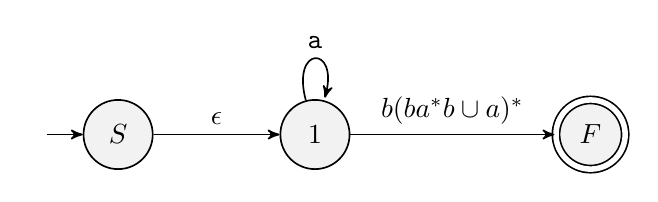
\begin{tikzpicture}
    
    \node[state, initial] (0) {$S$};
    \node[state, right of=0] (1) {$1$};
    \node[state, right of=1, accepting, xshift=1cm] (2) {$F$};
    
    \draw (0) edge node {\tt $\epsilon$} (1);
    \draw (1) edge node {\tt $b(ba^*b \cup a)^*$} (2);
    
    \draw (1) edge[loop above] node {\tt a} (1);
    
    \end{tikzpicture}
    
    ~\\~\\
    
    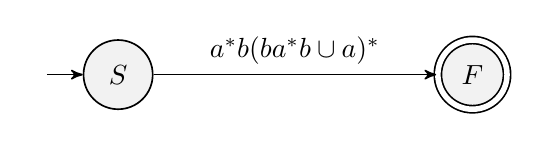
\begin{tikzpicture}
    
    \node[state, initial] (0) {$S$};
    \node[state, right of=0, accepting, xshift=2cm] (1) {$F$};
    
    \draw (0) edge node {\tt $a^*b(ba^*b \cup a)^*$} (1);
    
    
    \end{tikzpicture}
\end{center}

\section*{1.29 b}

\quad Assume that $A = \{www \:|\: w \in \{a, b\}^*\}$ is regular and let $p$ be the constant for which the pumping lemma holds for $A$.

\vspace{5mm} 

Let $w = a^nb^n = a^pb^p$ given the constant $p$ and then let $w' = a^pb^pa^pb^pa^pb^p$ where there are 3 identical copies of the word $w$ in a row.

\vspace{5mm} 

Then $w'$ is divided into $w' = xyz$ such that $|xy| \leq p$, $|y| \geq 1$, and $(\forall i \geq 0)[xy^iz \in A]$. By these definitions, y can only be composed of the symbol $a$ since the first $p$ symbols of $w'$ is composed of $a$'s and $|xy|$ is at most $p$ symbols long.

\vspace{5mm}

Then for any $i \neq 1$, we would have $a^qb^pa^pb^pa^pb^p$ where $ q \neq p$ and therefore the word $w'$ cannot be decomposed as three identical substrings $www$. This is a contradiction and thus the language $A$ is not regular.

\section*{1.40 b}

Suppose the language $A$ is regular. Then we can construct an NFA $N$ that recognizes $A$. We can apply a simple modification to $N$ to have it recognize $\textrm{NoExtend(A)}$. Since $\textrm{NoExtend(A)}$ is recognized by an NFA, lets call it $N'$, it is regular. Therefore, the class of regular languages is closed under the $\textrm{NoExtend()}$ operation.\\\\
Given the NFA $N = (Q, \Sigma, \delta, q_0, F)$ that recognizes $A$, we construct $N' = (Q', \Sigma', \delta', q_0', F')$ that recognizes $\textrm{NoExtend(A)}$ where 
\begin{itemize}
    \item $Q' = Q \cup \{q_f\}$ : we add one additional state to $Q$ and make it the one and only final state.
    \item $\Sigma' = \Sigma$ : we keep the same alphabet.
    \item $\delta' = \delta \cup \delta_\textrm{new}$ : we keep all of the old transitions but add some new ones. Out of every state, we add a arrow for every letter in $\Sigma$ that the state did not already have leaving it. This arrow then leads to $q_f$. This causes the automata to enter the accept state as soon as it reads a character that confirms the string is not a substring of any word accepted by $N$.
    \item $q_0' = q_0$ : we keep the same start state
    \item $F' = \{q_f\}$ : we make the set of accept states our new state.
\end{itemize}

\end{document}
